\section{Results}\label{sec:results}

\subsection{Attacker economics: finality dominates}\label{sec:res-attacker}

The bank core holds the most reachable value in \cref{tab:venues}, yet it is the only venue with a negative expected payoff, \payBank{} per attack. The cross-chain bridge offers \payBridge{}, the custodial exchange \payExchange{} and retail wallet campaigns \payWallet{} (\cref{fig:attacker}a). A rational attacker therefore prefers the bridge although it holds 40\% less value than the bank.

\Cref{prop:decomp} attributes the difference. The bridge's retained value is $e^{\gapTotal} = \retainedRatio$ times the bank's. Of the log gap of $\gapTotal$, finality contributes $\gapFinality$ (\shareFinality\%), a higher breach probability $\gapBreach$ (\shareBreach\%) and cheaper laundering $\gapLaundering$ (\shareLaundering\%), while the bridge's smaller balance works in the opposite direction, $\gapValue$ ($\shareValue$\%). Finality alone more than offsets the bank's balance-sheet advantage (\cref{fig:attacker}c). \Cref{cor:breakeven} turns this into a deterrence threshold: the bank remains unattractive as long as its recovery probability exceeds $\kappa^\ast = \breakEven$, and below that value its expected payoff rises linearly at \$6 million for every ten percentage points of recovery lost (\cref{fig:attacker}b). In this model the most effective defence of the banking core is not a harder perimeter but the ability to reverse what gets through.

\begin{figure}[!tbp]
\centering
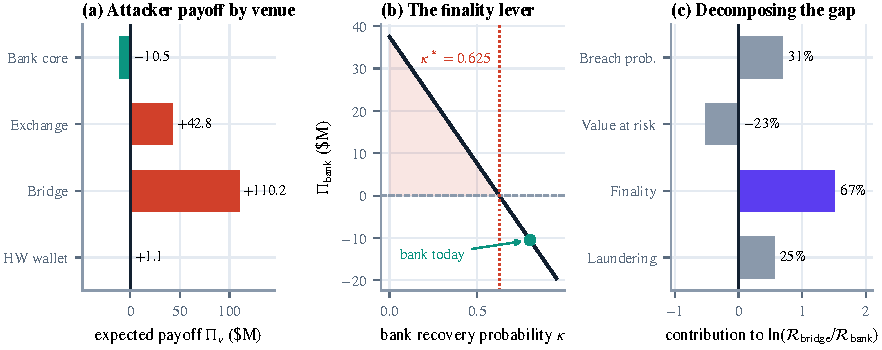
\includegraphics[width=\textwidth]{figures/fig2_attacker.pdf}
\caption{Attacker economics. (a) Risk-adjusted expected payoff $\Pi_v$ by venue, \cref{eq:payoff}. (b) The bank's payoff to an attacker as a function of its recovery probability $\kappa$; the bank is unattractive above the break-even value $\kappa^\ast$ of \cref{cor:breakeven}. (c) Exact decomposition of the log retained-value gap between bridge and bank, \cref{prop:decomp}; labels give each factor's share of the total.}
\label{fig:attacker}
\end{figure}

\subsection{Loss benchmarks and the compound-sum correction}\label{sec:benchmark}

In a 200{,}000-year run of the loss process, the mean annual loss is \ldaMean{} and the median \ldaMedian{}; the 95\%, 99\% and 99.9\% value-at-risk levels are \ldaVaRA{}, \ldaVaRB{} and \ldaVaRC{}, and the 99.9\% expected shortfall is \ldaESC{}, two and a half times the corresponding value-at-risk and close to the ratio $\alpha/(\alpha-1) \approx 2.67$ implied by a Pareto tail (\cref{fig:loss}). The truth used in the coverage study comes from a separate run of \TruthYears{} years: the 1-in-100-year annual loss is \truthC{}, the 1-in-1,000-year loss \truthK{}, and a year with losses of at least \$20 billion occurs on average once every \truthSys{} years, or with a probability of about half a percent per decade.

\Cref{app:shift} can be checked on the 200{,}000-year record. Above its 99.5th percentile (\fullU), the record contains \fullK{} exceedances, and the fitted shape is $\hat\xi = \fullXi$ (standard error \fullXiSE): with this much data, the estimate is precise but pulled below the planted \xiTrue{} by the log-normal body (\cref{rem:kink}). At $T = 100$ the incident-level return level \fullIncC{} misses the true annual level by \fullIncErrC\%; adding the mean annual loss of \fullShift{} gives \fullAggC, an error of \fullAggErrC\%. At $T=1{,}000$ the correction is only about 3\% of the level, and the remaining error (\fullIncErrK\% before, \fullAggErrK\% after) is governed by $\hat\xi$. This is the pattern \cref{eq:shift} predicts: the correction is first-order relevant at moderate return periods and second-order at long ones.

\begin{figure}[!tbp]
\centering
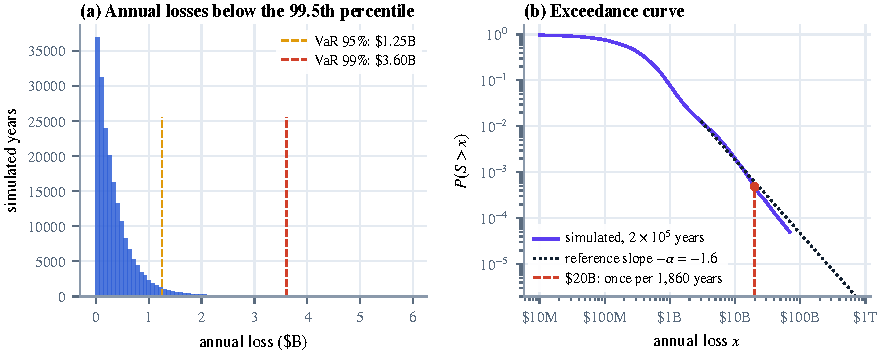
\includegraphics[width=\textwidth]{figures/fig3_loss.pdf}
\caption{The loss process. (a) Histogram of annual losses below the 99.5th percentile in a 200{,}000-year run, with value-at-risk levels. (b) Empirical exceedance curve on log--log axes; the dotted reference line has the planted slope $-\alpha$.}
\label{fig:loss}
\end{figure}

\subsection{What one record can and cannot reveal}\label{sec:single}

\Cref{fig:evt} shows inference from single records. Panels (a) and (b) use a 1,000-year record, more data than any real cyber-loss database. The mean-excess plot is close to linear, as a generalized Pareto tail requires, and the Hill estimate hovers near the planted $\alpha = 1.6$ over a range of moderate $k$. Yet the standard recipe of fitting at the 98th percentile places the threshold at \longU, just below the cascade trigger, and returns $\hat\xi = \longXi$ with a 95\% interval of $[\longXiLo, \longXiHi]$; the implied 1-in-1,000-year loss, \longPsi{}, is more than twice the truth. In the largest order statistics, where cascaded incidents dominate, the Hill estimate drifts towards one. A long record does not protect against a threshold placed on a kink.

Panel (c) uses a 100-year record with \shortK{} exceedances above \shortU{}, a typical draw with $\hat\xi = \shortXi$ close to the planted value. The point estimate of the 1-in-1,000-year loss is \shortPsi{} against a truth of \truthK{}. The three 95\% intervals are $[\shortDeltaLo, \shortDeltaHi]$ for the delta method, $[\shortBootLo, \shortBootHi]$ for the bootstrap and $[\shortProfileLo, \shortProfileHi]$ for the profile likelihood. All contain the truth here, but they disagree about where the uncertainty lies: the profile interval's lower limit is twice as high and its upper limit an order of magnitude higher. Panel (c) also exposes a pathology of the delta method. Its lower limit \emph{falls} as the return period grows beyond about a century, so that the lower confidence bound for the 1-in-10,000-year loss lies below the bound for the 1-in-100-year loss. This is the mechanical consequence of a log-symmetric band whose width grows faster than its centre. Profile limits are monotone in $T$, as they must be.

\begin{figure}[!tbp]
\centering
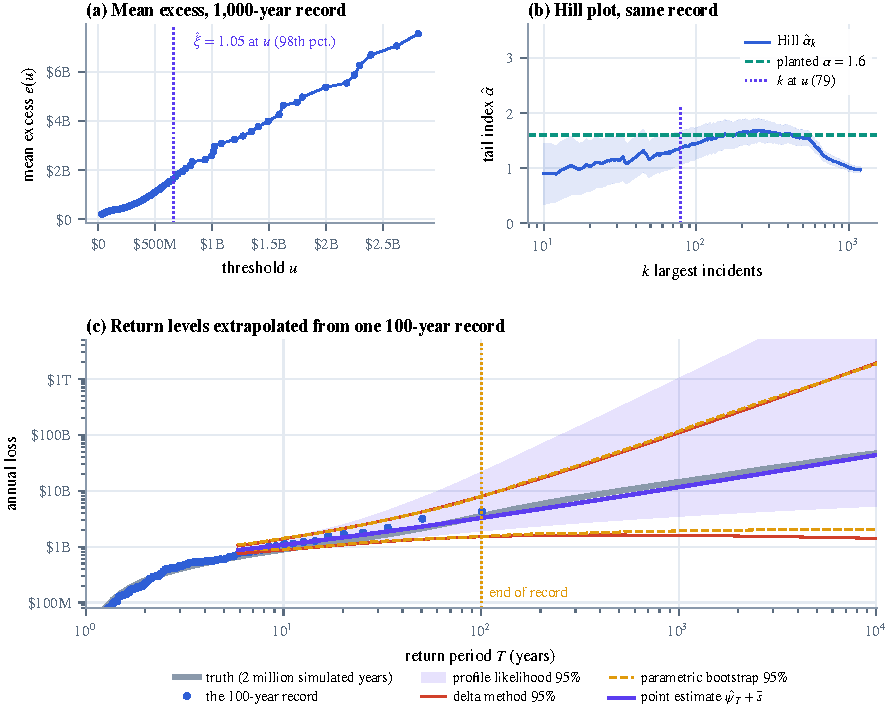
\includegraphics[width=\textwidth]{figures/fig4_evt.pdf}
\caption{Inference from single records. (a) Mean-excess plot of a 1,000-year record; the dotted line marks the 98th-percentile threshold. (b) Hill estimates $\hat\alpha_k$ with pointwise 95\% bands for the same record; the dashed line is the planted index. (c) Return levels from one 100-year record: the truth from \TruthYears{} simulated years, the record's own annual losses at their empirical return periods, the point estimate $\hat\psi_T + \bar s$, and 95\% intervals from the three methods.}
\label{fig:evt}
\end{figure}

\subsection{Coverage: how often is the truth inside?}\label{sec:coverage}

\Cref{tab:coverage} reports coverage for the 1-in-1,000-year loss, \cref{tab:misses} dissects the misses, and \cref{fig:coverage} shows all cells including $T=100$; \cref{tab:full} in the appendix gives every metric. Five findings stand out.

\emph{First, with records of realistic length the standard intervals fail.} In the full pipeline with 30-year records, the delta method covers the true 1-in-1,000-year loss \covBThirtyDeltaK\% of the time and the bootstrap \covBThirtyBootstrapK\%; with 100-year records these rise only to \covBHundredDeltaK\% and \covBHundredBootstrapK\%. The failure is not caused by misspecification: in Experiment A, where the model is exactly right, the delta method covers \covAThirtyDeltaK\% with 15 exceedances and \covAHundredDeltaK\% with 50. The parametric bootstrap, often recommended as a remedy, does no better: its coverage is within about two percentage points of the delta method's in every short-record cell.

\emph{Second, the failures are one-sided and dangerous.} Virtually every miss of the delta and bootstrap intervals lies wholly below the truth: \belowBThirtyDeltaK\% of delta intervals in the 30-year pipeline cell and \belowAThirtyDeltaK\% in the corresponding cell of Experiment A, with none lying above it (\cref{tab:misses}). These intervals do not merely understate uncertainty; they understate the loss.

\emph{Third, the cause is a downward-biased point estimate.} The median estimate of the 1-in-1,000-year loss is \medRatioBThirtyK{} times the truth with 30-year records in the pipeline and \medRatioAThirtyK{} times the truth in Experiment A, recovering to \medRatioAHundredK{} and \medRatioAThreeHundredK{} with 50 and 150 exceedances. The mechanism is the skewness of $\hat\xi$ in small samples from heavy tails: a short record rarely contains the extreme incidents that reveal how heavy the tail is, so $\hat\xi$ is below $\xi$ more often than not, and because $\psi_T$ increases steeply in $\xi$ when $\lambda_u T$ is large, $\operatorname{median}(\hat\psi_T)\approx\psi_T(\operatorname{median}\hat\xi) < \psi_T$. Any interval that is symmetric on the log scale around such an estimate inherits the bias.

\emph{Fourth, profile likelihood repairs most of the damage, and is better by a proper score.} Profile-likelihood intervals, which can be strongly right-skewed, cover \covBThirtyProfileK\% and \covBHundredProfileK\% in the 30- and 100-year pipeline cells and \covAThirtyProfileK\%, \covAHundredProfileK\% and \covAThreeHundredProfileK\% in Experiment A. Every short-record improvement over both alternatives is significant in a paired McNemar test ($p<0.001$). Coverage gains could in principle come from indiscriminately wide intervals, but the interval score rules this out: the profile likelihood roughly halves the mean score in the 30-year cells (\scoreBThirtyProfileK{} against \scoreBThirtyDeltaK{} for the delta method and \scoreBThirtyBootstrapK{} for the bootstrap in Experiment B) and has the lowest score in every cell of Experiment A. The price of honesty is width where data are thin: with 15 exceedances the median profile interval spans a factor of \ratioAThirtyProfileK{} from lower to upper limit, against \ratioAThirtyDeltaK{} for the delta method. With 150 exceedances the three methods converge (coverage \covAThreeHundredDeltaK\%, \covAThreeHundredBootstrapK\% and \covAThreeHundredProfileK\%; width ratios \ratioAThreeHundredDeltaK, \ratioAThreeHundredBootstrapK{} and \ratioAThreeHundredProfileK).

\emph{Fifth, no interval method fixes a biased threshold.} With 1,000-year records the threshold rule places $u$ near the cascade kink and the median estimate overshoots the truth by a factor of \medRatioBThousandK{}. The profile likelihood's misses then flip to the conservative side: only \belowBThousandProfileK\% of its intervals lie below the truth, and its coverage of \covBThousandProfileK\% is now significantly lower than that of the delta method (\covBThousandDeltaK\%), whose log-symmetric lower half happens to catch an overestimated level. The interval score agrees (\scoreBThousandProfileK{} against \scoreBThousandDeltaK{}). This cell is a reminder that interval calibration and threshold choice are separate problems: the first is solved by the profile likelihood, the second requires diagnostics and sensitivity analysis.

\begin{table}[!tbp]
\centering\small
\begin{threeparttable}
\caption{Coverage of nominal 95\% intervals for the 1-in-1,000-year loss}\label{tab:coverage}
\setlength{\tabcolsep}{5pt}
\begin{tabular}{@{}lrrrccc@{}}
\toprule
Experiment & $R$ (years) & $\bar k$ & Median $\hat\psi/\psi$ & Delta method & Bootstrap & Profile LR \\
\midrule
\tabinput{tables/tab_coverage_main.tex}
\bottomrule
\end{tabular}
\begin{tablenotes}\footnotesize
\item \emph{Notes:} Coverage in percent over \Reps{} independent records per row, with 95\% Wilson intervals in brackets. $\bar k$ is the mean number of exceedances; median $\hat\psi/\psi$ is the median ratio of the point estimate to the truth. Experiment A: exceedances exactly generalized Pareto with $\xi = \xiTrue$, truth \truthAK. Experiment B: full loss pipeline with thresholds at the 85th, 95th and 98th percentiles, truth \truthK.
\end{tablenotes}
\end{threeparttable}
\end{table}

\begin{table}[!tbp]
\centering\footnotesize
\begin{threeparttable}
\caption{Anatomy of the misses, 1-in-1,000-year loss}\label{tab:misses}
\setlength{\tabcolsep}{3.6pt}
\begin{tabular}{@{}lrrrrrrrrrrrr@{}}
\toprule
 & & \multicolumn{3}{c}{Below truth (\%)} & \multicolumn{3}{c}{Median upper/lower} & \multicolumn{3}{c}{Interval score} & \multicolumn{2}{c}{McNemar $p$} \\
\cmidrule(lr){3-5}\cmidrule(lr){6-8}\cmidrule(lr){9-11}\cmidrule(l){12-13}
Exp. & $R$ & Delta & Boot. & Profile & Delta & Boot. & Profile & Delta & Boot. & Profile & P vs D & P vs B \\
\midrule
\tabinput{tables/tab_misses.tex}
\bottomrule
\end{tabular}
\begin{tablenotes}\footnotesize
\item \emph{Notes:} ``Below truth'' is the share of intervals lying wholly below the true loss. The interval score is \cref{eq:score} on the $\log_{10}$ scale with $\alpha = 0.05$ (lower is better). McNemar $p$ is the exact two-sided $p$-value for the paired difference in coverage between the profile likelihood (P) and the delta method (D) or the bootstrap (B).
\end{tablenotes}
\end{threeparttable}
\end{table}

\begin{figure}[!tbp]
\centering
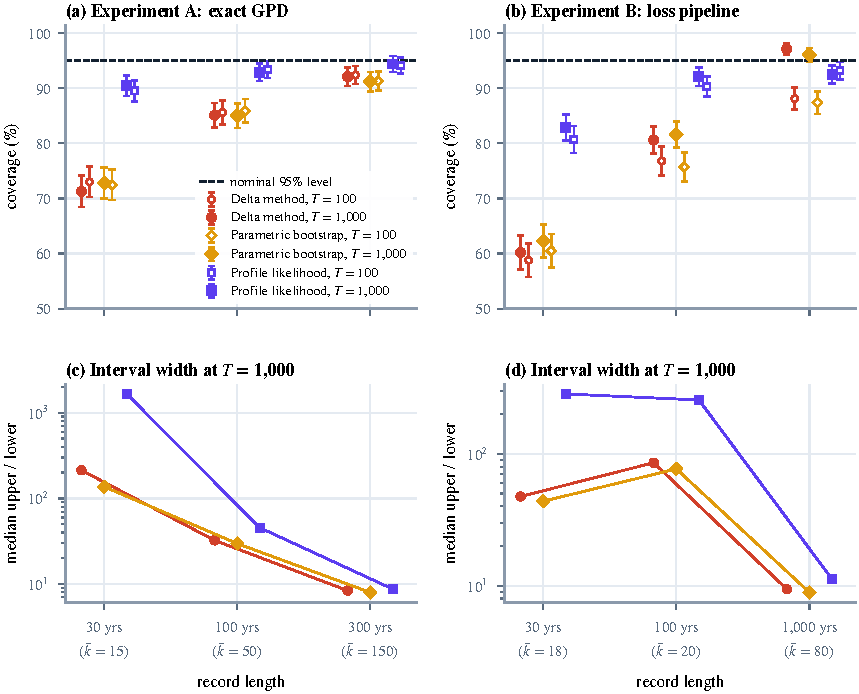
\includegraphics[width=\textwidth]{figures/fig5_coverage.pdf}
\caption{Coverage study. (a, b) Coverage of nominal 95\% intervals with 95\% Monte Carlo error bars, for $T = 1{,}000$ (filled) and $T = 100$ (open); the dashed line marks the nominal level. (c, d) Median ratio of upper to lower limit at $T = 1{,}000$ on a log scale. Experiment A fits a correctly specified tail above a known threshold; Experiment B runs the full pipeline on records from the loss process.}
\label{fig:coverage}
\end{figure}

\subsection{Contagion: a phase transition, and importance without size}\label{sec:res-contagion}

The exposure matrix of the network has $\rho(\Omega W) = \rhoOne$, so by \cref{prop:debtrank} shocks stop dying out once interbank exposure exceeds $\ell^\ast = \critExp$ times equity. \Cref{fig:contagion}a shows the transition. Below $\ell^\ast$ the contagion multiplier grows smoothly as the system approaches criticality; at $\ell^\ast$ it jumps by an order of magnitude and then saturates as every reachable bank defaults. At $\ell = 0.5$ a cyber event that wipes out 20\% of the largest bank's equity causes direct losses of \scBigDirect{} and total losses of \scBigTotal{} ($\Mult = \scBigMult$) without any default (\cref{tab:scenarios}). The same exposure scale makes a shared-vendor event benign: eight banks lose \scVendLowDirect{} directly and the system \scVendLowTotal{} in total. At $\ell = 1.2$, the vendor event destroys \scVendHighTotal, \scVendHighShare\% of system equity, and \scVendHighDef{} of the \nBanks{} banks default. The danger of concentration in third-party technology is not visible in calm, subcritical conditions; it materializes abruptly once leverage crosses a threshold.

\enlargethispage{\baselineskip}% final layout: lets the Discussion heading start on this page
Systemic importance, measured by the multiplier when a bank alone is hit, does not follow size (\cref{fig:contagion}b and \cref{tab:ranking}). The most systemic bank, \topOneName{} ($\Mult = \topOneMult$), is the smallest of the five core banks, and the second, \topTwoName{} ($\Mult = \topTwoMult$), is a periphery bank ranked \pOneSizeRank{}nd of \nBanks{} by assets that outranks \pOneBeatsCore{} core banks \pOneRatioLo{} to \pOneRatioHi{} times its size. The distinction between amplification and absolute impact matters here: a hit on the largest bank still produces the largest total loss (\scBigTotal{} against \cOneTotal{} for \topOneName{} and \pOneTotal{} for \topTwoName{}), but per dollar of direct damage, interconnection rather than size determines how far losses travel. Supervisory metrics that rank institutions by size alone will miss banks whose creditors are themselves thinly capitalized and densely connected.

\begin{table}[!tbp]
\centering\small
\begin{threeparttable}
\caption{Contagion scenarios (shock: 20\% of the equity of each bank hit)}\label{tab:scenarios}
\begin{tabular}{@{}lrrrrr@{}}
\toprule
Scenario & Direct loss & Total loss & $\Mult$ & Defaults & Rounds \\
\midrule
\tabinput{tables/tab_scenarios.tex}
\bottomrule
\end{tabular}
\begin{tablenotes}\footnotesize
\item \emph{Notes:} $\ell$ is the exposure scale; the critical value is $\ell^\ast = \critExp$. Total system equity is \sysEquity. Rounds count propagation steps until the relative change falls below $2\times10^{-4}$.
\end{tablenotes}
\end{threeparttable}
\end{table}

\begin{table}[!tbp]
\centering\small
\begin{threeparttable}
\caption{Most systemic banks by contagion multiplier ($\ell = 0.5$, 20\% equity shock)}\label{tab:ranking}
\begin{tabular}{@{}rllrrr@{}}
\toprule
Rank & Bank & Tier & Assets (\$B) & Size rank & $\Mult$ \\
\midrule
\tabinput{tables/tab_ranking.tex}
\bottomrule
\end{tabular}
\end{threeparttable}
\end{table}

\begin{figure}[!tbp]
\centering
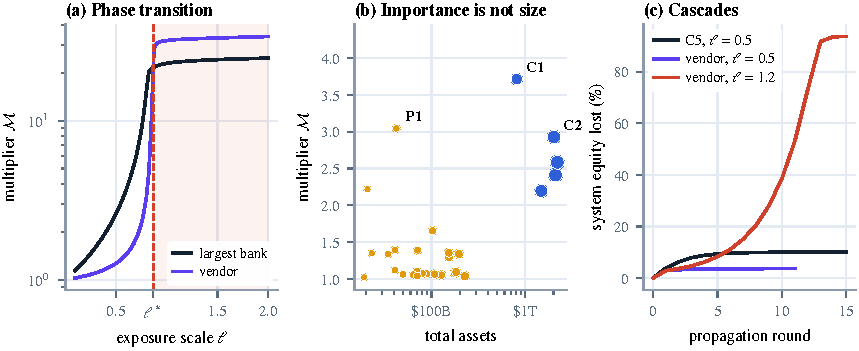
\includegraphics[width=\textwidth]{figures/fig6_contagion.pdf}
\caption{Interbank contagion. (a) Contagion multiplier $\Mult$ against the exposure scale $\ell$ for a hit on the largest bank and on a shared vendor serving eight banks; the dashed line marks $\ell^\ast = 1/\rho(\Omega W)$ and the shaded region the supercritical regime. (b) Multiplier when each bank alone is hit, against total assets; core banks in blue, periphery banks in amber. (c) Share of system equity lost by propagation round.}
\label{fig:contagion}
\end{figure}
